\section{Miscellaneous Notes}
% the text width in a normal line is 11.80737cm
% To make a TODO note, start a comment with two or more consecutive capital letters.
% I use the svgnames xcolor scheme. Find a table of names at:
% https://www.latextemplates.com/svgnames-colors

\section{Captions and Labels}
%  All lables begin with the following (as appropriate).
%	ch: -- chapter
%	sec: -- section
%	subsec: -- sub-section
%	para: -- paragraph
%	tab: -- table
%	eq: -- equation
%	fig: -- figure
%	lst: -- code listing
%	soln: -- the solution to an equation
%	A full label would look something like: \label{03:tab:truth_table_for_or}

% My standard is:
% Circuit/Subcircuit name: \lstinline[columns=fixed]|main|
% Input/Output Pin: italics
% Tools (like poke): italics
% Devices (like constants) in a format like: Constant (\textit{Wiring} library)
% Menu items should be in small caps: \textsc{Simulate -> Reset Simulation}
% Gates should be in all caps and typewriter font: \texttt{AND}
% Signals should be italicised in typewriter font: \textit{\texttt{Activate}}

% The word subcircuit is not hyphenated
% Logisim-evoluation is capitalized and placed in italics: \textit{Logisim-evolution}
% Boolean equations are written as math equations

\section{My Macros}
None

%************************************************************
\section{acronyms}
% Define a new acronym in "Contents.tex"
% The definition takes the form: \acro{POS}{Product of Sums}
% Enter them in alphabetic order since they will be printed in the Table of Acronymns 
% 	in the same order that they are listed on the Contents page
%***************************************************************
\ac{ACR}   % prints the acronym text and then the acronym in brackets 
\acl{ACR}  % prints the long version (the definition without acronym)
\acf{ACR}  % prints the full name of the acronym plus the acronym
\acs{ACR}  % prints the short version (no definition)
\acp{ACR}  % prints the plural version
\acfp{ACR} % prints the full version in plural
\aclp{ACR} % prints the long version in plural

%*****************************************************
\section{Truth Table}
%*****************************************************
\begin{table}[H]
	\sffamily
	\newcommand{\head}[1]{\textcolor{white}{\textbf{#1}}}		
	\begin{center}
		\rowcolors{2}{gray!10}{white} % Color every other line a light gray
		\begin{tabular}{ccc} 
			\rowcolor{black!75}
			\multicolumn{2}{c}{\head{Inputs}} & \head{Output} \\
			A & B & Y \\
			\hline
			0 & 0 & 0 \\
			0 & 1 & 1 \\
			1 & 0 & 1 \\
			1 & 1 & 1 
		\end{tabular}
	\end{center}
	\caption{Truth Table for OR}
	\label{tab:intro-01}
\end{table}


%******************************************************
\section{3-Line Equation}
%******************************************************
\begin{align}
	\label{03:eq:identity_example}
	1101_2 &= 123 \\
	\nonumber
	&= 123 \\
	\nonumber
	&= 123
\end{align}


\section{Solving an Equation Step-by-step}
\begin{align}
	\label{04:soln:solving_equation_one}
	AB+BC(B+C) && \text{Original Expression} \\
	\nonumber
	AB+BBC+BCC && \text{Distribute BC} \\
	\nonumber
	AB+BC+BC && \text{Idempotence: BB=B and CC=C} \\
	\nonumber
	AB+BC && \text{Idempotence: BC+BC=BC} \\
	\nonumber
	B(A+C) && \text{Factor} \\
\end{align}

%**************************************************************************
\section{Margin Paragraph} 
%**************************************************************************
\marginpar{Whatever.}

%***************************************************************************
\section{Comment Box}
%***************************************************************************
\begin{tcolorbox}[colback=blue!5!white,colframe=blue!75!black]
	% Upper half of box: my "title" area
	\textcolor{blue}{\textbf{Interesing Note}}
	% Lower half of the box: the content
	\tcblower
	Whatever.
\end{tcolorbox}

%***************************************************************************
\section{Insert Figure}
%***************************************************************************
\begin{figure}[H]
	\centering
	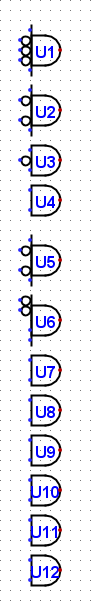
\includegraphics[width=\maxwidth{.95\linewidth}]{gfx/03-01}
	\caption{Caption}
	\label{fig:03-01}
\end{figure}

%****************************************************
\section{Verbatim Section}
%****************************************************
\begin{Verbatim}[frame=lines,
                 numbers=left,
                 xleftmargin=10mm,
                 xrightmargin=10mm]
Text goes here...
\end{Verbatim}


%****************************************************
\section{Verilog Code Snip}
%****************************************************
\lstset{ %
  caption={caption},
  label=SL:lst:listing01,
  numbers=left,
  language=Verilog
}
\begin{lstlisting}
  Code here
\end{lstlisting}

%***************************************************************************
\section{Verilog From File For Text Area}
%***************************************************************************
\lstset{ %
  caption={add2 Solution},
  label=L03:lst:add2,
  basicstyle={},
  upquote=false, 
  numbers=left,
  language=Verilog
}
\lstinputlisting[firstline=7]{ckt/lab03.add2.v}

\section{Verilog From File For Code Snip}
%***************************************************************************
\lstset{ %
  caption={add2 Solution},
  label=L03:lst:add2,
  basicstyle={\ttfamily},
  upquote=true,
  numbers=none,
  language=teX
}
\lstinputlisting[firstline=7]{ckt/lab03.add2.v}

%***************************************************************************
\section{Timing Table}
%***************************************************************************
\begin{figure}[H]
  \centering
  \begin{tikztimingtable}[
    timing/slope=0,         % no slope
    timing/coldist=2pt,     % column distance
    xscale=2.0,yscale=1.0,  % scale diagrams
    semithick,               % set line width
    ]
    \footnotesize \# & U     R 8{2Q} 2U     \\
    \footnotesize Clk & 17{C} \\
    %                     P 01 02 03 04 05 06 07 08
    \footnotesize E & [] {H HH HH HH HH LL LL LL LL} \\
    \footnotesize S & [] {H HH LL HH LL HH LL LL HH} \\
    \footnotesize Q & [] {H HH LL HH LL HH HH HH HH} \\
    \extracode % Optional
    % \fulltablegrid[]
    % \vertlines[]{}
    \tablerules[]
  \end{tikztimingtable}
  \caption{D Latch Timing Diagram} 
  \label{SL:fig:d_latch_timing_diagram}
\end{figure}


%***************************************************************************
\section{Lorem Ipsum}
%***************************************************************************
\lipsum[1] % Number of paragraphs can be specified

%***************************************************************************
\section{Listing In Line}
%***************************************************************************
\lstinline[columns=fixed]|code|


%***************************************************************************
\section{Wrap Figure}
%**************************************************************************
\begin{wrapfigure}{O}{0.2\textwidth}
	\caption{} % No text, wraps badly in very narrow space (does print fig number)
	\label{BM:fig:gray_code_disc} 
	\centering
	\includegraphics[width=0.2\textwidth]{gfx/gray_code_disc} 
\end{wrapfigure}


%***************************************************************************
\section{Regular Figure}
%**************************************************************************
\begin{figure}[H]
  \centering
  \frame{\includegraphics{ckt/lab_hello.png}}
  \caption{Executing ``Hello World''}
  \label{fig:intro-01}
\end{figure}

\section{Circuit Diagram}
% Node Notes:
% \node[and  gate,inputs={nn},anchor=east] (g01) at (2.00,2.00) {};
%	inputs can be "n" (normal) or "i" (inverted) and you can put as many as needed (with some exceptions,
%	  for example, XOR gates can only have two inputs so the first two are accepted and any others ignored). 
%	For consistency and ease in design, anchor all gates "east" (that is the output port).
%	All gates are named by simply numbering from "g01" up. That makes it much easier to copy/paste a
%	  diagram since you don't have to re-name all of the gates.
%	While designing the circuit, put the gate number in the braces at the end of the line. That will
%	  print the gate number on the gate itself so it is easier to run wires from one gate to the next.
% Measurements:
%	The measures are (horizontal,vertical), or (X,Y)
%	The anchor point is the output of the gate.
%	The two inputs are 0.1 above and below the anchor
%	Thus, if an AND gate is at (1.00,1.00), line up two inputs by locating them at (0.00,1.10) and (0.00,0.90)
%	Two one-above-the-other gates on the diagram can be 1.00 apart without overlap. Thus, two vertically 
%	  stacked AND gates can be at (1.00,1.00) and (1.00,2.00).
%	Two side-by-side gates on the diagram can be 1.50 apart without overlap. Thus, two AND gates on the same row can 
%	  be at (1.00,1.00) and (2.50,1.00).
% Names:
%	g01 for gates
%	n01 for inputs
%	c01 for connectors
%	y01 for outputs
% Input Labels:
%	The system will only allow labels at the 8 compass corners (west, south west, south, etc.). For brevity,
%	  I use degrees rather than the compass words. 0 degrees is "east".
%	I prefer all labels to be at 180 degrees ("west"). To offset that label so it doesn't interfere with
%	  another label above or below, use 150 to move it to "north west" and 210 to move it to "south west"
\begin{figure}[H]
	\caption{Grouping With DeMorgan's Theorem}
	\label{03:fig:grouping_with_demorgans_theorem}	
	\myfloatalign
	\begin{tikzpicture} [circuit logic US, scale=1.00]
	% make all path lines (the node shapes) a little thicker
	\tikzstyle{every path}=[line width=0.50mm]	
	
	% Logic Gates
	\node[and  gate,inputs={nn},anchor=east] (g01) at (2.00,2.00) {};
	\node[nand gate,inputs={ni},anchor=east] (g02) at (2.00,1.00) {};
	\node[nor  gate,inputs={nn},anchor=east] (g03) at (3.50,2.50) {};
	\node[nor  gate,inputs={nn},anchor=east] (g04) at (5.00,1.50) {};
	% Input nodes
	\node[circ,label={180:A}] (nA) at (0.0,2.60) {};
	\node[circ,label={180:B}] (nB) at (0.0,2.10) {};
	\node[circ,label={210:C}] (nC) at (0.0,1.90) {};
	% Connector Nodes
	\node[circ] (c01) at (0.5,2.10) {};
	\node[circ] (c02) at (0.3,1.90) {};	
	% Output nodes
	\node[circ,label={0:Y}] (y01) at (5.50,1.50) {};
	
	% Draw the lines
	\draw
		(nA) -- (g03.input 1)
		(nB) -- (c01) -- (g01.input 1)
		(c01) |- (g02.input 1)
		(nC) -- (c02) -- (g01.input 2)
		(c02) |- (g02.input 2)
		(g01.output) -- (2.25,2.00) |- (g03.input 2)
		(g03.output) -- (3.75,2.50) |- (g04.input 1)
		(g02.output) -- (3.75,1.00) |- (g04.input 2)
		(g04.output) -- (y01)
	;		
	\end{tikzpicture}
\end{figure}

% *****************************************************
\section{Karnaugh Map For 4-Input Circuit}
% *****************************************************

\begin{figure}[H]
  \myfloatalign
  \begin{tikzpicture} [circuit logic US, scale=1.00]
  % make all path lines (the node shapes) a little thicker
  \tikzstyle{every path}=[line width=0.50mm]
  
  %********************************************************************
  % Adjust the settings below to display the 1's and rectangles
  %********************************************************************
  % Uncomment the appropriate lines below to insert ones where needed
  % Data Row 1
  % \node[] at (2.25,5.25) {\Huge $ 1 $}; % 00
  % \node[] at (3.75,5.25) {\Huge $ 1 $}; % 04
  % \node[] at (5.25,5.25) {\Huge $ 1 $}; % 12
  % \node[] at (6.75,5.25) {\Huge $ 1 $}; % 08
  % Data Row 2
  % \node[] at (2.25,3.75) {\Huge $ 1 $}; % 01
  % \node[] at (3.75,3.75) {\Huge $ 1 $}; % 05
  \node[] at (5.25,3.75) {\Huge $ 1 $}; % 13
  % \node[] at (6.75,3.75) {\Huge $ 1 $}; % 09
  % Data Row 3
  % \node[] at (2.25,2.25) {\Huge $ 1 $}; % 03
  % \node[] at (3.75,2.25) {\Huge $ 1 $}; % 07
  \node[] at (5.25,2.25) {\Huge $ 1 $}; % 15
  \node[] at (6.75,2.25) {\Huge $ 1 $}; % 11
  % Data Row 4
  % \node[] at (2.25,0.75) {\Huge $ 1 $}; % 02
  % \node[] at (3.75,0.75) {\Huge $ 1 $}; % 06
  % \node[] at (5.25,0.75) {\Huge $ 1 $}; % 14
  % \node[] at (6.75,0.75) {\Huge $ 1 $}; % 10
  
  % The coords for each cell - this is used to start the rectangle box
  \coordinate (cell00) at (1.50,4.50); \coordinate (cell01) at (1.50,3.00);
  \coordinate (cell02) at (1.50,0.00); \coordinate (cell03) at (1.50,1.50);
  \coordinate (cell04) at (3.00,4.50); \coordinate (cell05) at (3.00,3.00);
  \coordinate (cell06) at (3.00,0.00); \coordinate (cell07) at (3.00,1.50);
  \coordinate (cell08) at (6.00,4.50); \coordinate (cell09) at (6.00,3.00);
  \coordinate (cell10) at (6.00,0.00); \coordinate (cell11) at (6.00,1.50);
  \coordinate (cell12) at (4.50,4.50); \coordinate (cell13) at (4.50,3.00);
  \coordinate (cell14) at (4.50,0.00); \coordinate (cell15) at (4.50,1.50);
  
  % Set the ``at'' to the lower-left cell of the rectangle using the coords defined above
  % Set the minimum height/width to (number of cells) * 1.5. May have to decrease 
  % these by 0.1 to cut the rectangle just inside the cell.
  \node [draw,
  color=red!70!black,
  fill=red!20!white,
  fill opacity=0.3,
  minimum height=1.4cm,
  minimum width=3.0cm,
  double,
  rounded corners,
  anchor=south west] at (cell15) {};
  \node [draw,
  color=blue!70!black,
  fill=blue!20!white,
  fill opacity=0.3,
  minimum height=2.9cm,
  minimum width=1.5cm,
  double,
  rounded corners,
  anchor=south west] at (cell15) {};
  
  %********************************************************************
  % Shouldn't need to adjust anything below this point - this is just
  % the grid and the minterms.
  %********************************************************************	
  % Text in top-Left cell
  \node[] at (0.55,6.35) { $ \mathsf{ \mathbf{CD} } $ }; % CD
  \node[] at (1.05,7.05) { $ \mathsf{ \mathbf{AB} } $ }; % AB
  
  % Populate the top row header
  % In the following, the foreach lists a location/text pair
  % The the draw line draws the text at each location
  \foreach \loc/\txt in {(2.25,6.75)/{00},(3.75,6.75)/{01},(5.25,6.75)/{11},(6.75,6.75)/{10}}
  \draw \loc node{\Huge $\txt$};
  
  % Populate the header in column one
  \foreach \loc/\txt in {(0.75,5.25)/{00},(0.75,3.75)/{01},(0.75,2.25)/{11},(0.75,0.75)/{10}}
  \draw \loc node{\Huge $\txt$};
  
  % Populate the minterms
  \foreach \loc/\txt in { (2.75,4.75)/{00} , (4.25,4.75)/{04} , (5.75,4.75)/{12} , (7.25,4.75)/{08} ,
    (2.75,3.25)/{01} , (4.25,3.25)/{05} , (5.75,3.25)/{13} , (7.25,3.25)/{09} ,
    (2.75,1.75)/{03} , (4.25,1.75)/{07} , (5.75,1.75)/{15} , (7.25,1.75)/{11} ,
    (2.75,0.25)/{02} , (4.25,0.25)/{06} , (5.75,0.25)/{14} , (7.25,0.25)/{10} }
  \draw \loc node{ \color{blue!90!black} \small{ $\txt$ }};
  
  % Draw the lines
  \draw
  % Finish drawing the grid
  [step=1.5cm,black,thin] (0,0) grid (7.5,7.5) % The Grid
  (0.0,7.5) -- (1.5,6.0) % Diagonal in the top left cell
  (1.5,6.10) -- (7.50,6.10) % Double line under top header row
  (1.40,0.0) -- (1.40,6.0) % Double line on left of header column one
  ;
  \end{tikzpicture}
  \caption{K-Map Example 1}
  \label{04:fig:kmap_01}
\end{figure}

\section{Generic IC}
%************************************************************************
% The following draws an adder as an IC and then defines five
% Input/Output nodes that will take connections from elsewhere. I can 
% use this type of circuit anywhere I need to create some sort of IC
% within a larger circuit.
%************************************************************************
\begin{figure}[H]
	\caption{4-Bit Adder}
	\label{CL:fig:4_bit_adder}	
	\myfloatalign
	\begin{tikzpicture} [circuit logic US, scale=1.00]
	% make all path lines (the node shapes) a little thicker
	\tikzstyle{every path}=[line width=0.50mm]	
	
	% Adder 1
	\node[minimum size=1.5cm,draw] (g01) at (2.00,8.00) {};
	\node[label={[label distance=-0.35cm]0:A}]   (n1a) at (1.40,8.25) {};
	\node[label={[label distance=-0.35cm]0:B}]   (n1b) at (1.40,7.75) {};
	\node[label={[label distance=-0.35cm]270:I}] (n1i) at (2.00,8.60) {};
	\node[label={[label distance=-0.35cm]90:O}]  (n1o) at (2.00,7.40) {};
	\node[label={[label distance=-0.35cm]180:S}] (n1s) at (2.60,8.00) {};
	
	% Adder 2
	\node[minimum size=1.5cm,draw] (g02) at (2.00,6.00) {};
	\node[label={[label distance=-0.35cm]0:A}]   (n2a) at (1.40,6.25) {};
	\node[label={[label distance=-0.35cm]0:B}]   (n2b) at (1.40,5.75) {};
	\node[label={[label distance=-0.35cm]270:I}] (n2i) at (2.00,6.60) {};
	\node[label={[label distance=-0.35cm]90:O}]  (n2o) at (2.00,5.40) {};
	\node[label={[label distance=-0.35cm]180:S}] (n2s) at (2.60,6.00) {};
	
	% Adder 3
	\node[minimum size=1.5cm,draw] (g03) at (2.00,4.00) {};
	\node[label={[label distance=-0.35cm]0:A}]   (n3a) at (1.40,4.25) {};
	\node[label={[label distance=-0.35cm]0:B}]   (n3b) at (1.40,3.75) {};
	\node[label={[label distance=-0.35cm]270:I}] (n3i) at (2.00,4.60) {};
	\node[label={[label distance=-0.35cm]90:O}]  (n3o) at (2.00,3.40) {};
	\node[label={[label distance=-0.35cm]180:S}] (n3s) at (2.60,4.00) {};
	
	% Adder 4
	\node[minimum size=1.5cm,draw] (g04) at (2.00,2.00) {};
	\node[label={[label distance=-0.35cm]0:A}]   (n4a) at (1.40,2.25) {};
	\node[label={[label distance=-0.35cm]0:B}]   (n4b) at (1.40,1.75) {};
	\node[label={[label distance=-0.35cm]270:I}] (n4i) at (2.00,2.60) {};
	\node[label={[label distance=-0.35cm]90:O}]  (n4o) at (2.00,1.40) {};
	\node[label={[label distance=-0.35cm]180:S}] (n4s) at (2.60,2.00) {};
		
	% Draw the lines
	\draw
	(n1o) -- (n2i)
	(n2o) -- (n3i)
	(n3o) -- (n4i)
	
	%	(nA) -- (g03.input 1)
	%	(nB) -- (c01) -- (g01.input 1)
	%	(c01) |- (g02.input 1)
	%	(nC) -- (c02) -- (g01.input 2)
	%	(c02) |- (g02.input 2)
	%	(g01.output) -- (2.25,2.00) |- (g03.input 2)
	%	(g03.output) -- (3.75,2.50) |- (g04.input 1)
	%	(g02.output) -- (3.75,1.00) |- (g04.input 2)
	%	(g04.output) -- (y01)
	;		
	\end{tikzpicture}
\end{figure}
